\documentclass[a4paper,12pt]{article}
\usepackage[utf8]{inputenc}
\usepackage{graphicx}
\usepackage{float}
\usepackage[spanish]{babel}
\usepackage{listings}
\usepackage{xcolor}
\definecolor{gris}{RGB}{123, 126, 132}
\definecolor{morado}{RGB}{81, 40, 155}
\definecolor{amarillo}{RGB}{253,151,31}
\definecolor{magenta}{RGB}{249,38,114}

\lstdefinestyle{customJava}{
    frame=tb,
    language=Java,
    backgroundcolor=\color{white},   
    commentstyle=\itshape\color{gris},
    keywordstyle=\bfseries\color{magenta},
    numberstyle=\color{morado},
    stringstyle=\color{amarillo},
    identifierstyle=\color{black},
    basicstyle=\footnotesize,
    breakatwhitespace=false,         
    breaklines=true,                 
    captionpos=b,
    keepspaces=true,                 
    numbers=left,                    
    numbersep=5pt,                  
    showspaces=false,                
    showstringspaces=false,
    showtabs=false,                  
    tabsize=2,
}

%opening
\title{Tarea No. 15. Patrón Front Controller y CDI}
\author{Barrera Pérez Carlos Tonatihu \\ Profesor: José Asunción Enríquez 
Zárate \\ Web Application Development \\ Grupo: 3CM9 }

\begin{document}

\maketitle
\newpage

\section{Desarrollo}
\subsection{Patrón front controller}
El patrón de diseño front controller significa que todas las peticiones que 
vienen por un recurso en una aplicación serán manejadas por un solo manejador y 
después serán enviadas al respectivo manejador dependiendo del tipo de 
solicitud. El front controller puede usar auxiliares para lograr el mecanismo 
de envío.

\begin{figure}[H]
    \begin{center}
    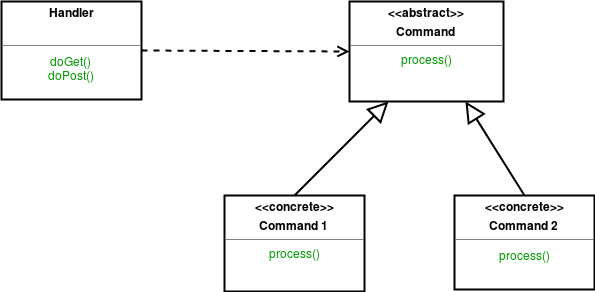
\includegraphics[width=\textwidth]{uml-front-controller-design-pattern.png}
    % estructura.png: 800x436 px, 96dpi, 21.16x11.53 cm, bb=0 0 600 327
    \caption{Patrón Front Controller}
    \label{fig:diagrama}
    \end{center}
\end{figure}
\subsubsection{Elementos del patrón}
\begin{itemize}
 \item Controlador. El controlador es el punto de contacto inicial para el 
manejo de las peticiones en el sistema. El controlador delega a un auxiliar 
para completar la autenticación y autorización de un usuario o para inicializar 
la recuperación de contactos.
\item Vista. Una vista representa y despliega información al cliente. La 
vista recupera información del modelo. Los auxiliares apoyan a las vistas 
mediante el encapsulado y adaptación del subyacente modelo de datos para su uso 
en la visualización.
\item Despachador. Es el responsable del manejo de las vistas y la 
navegación, manejando la elección de la siguiente vista a presentar al usuario, 
y proveyendo el mecanismo para el control de vectores de este recurso.
\item Auxiliar. Es el responsable de ayudar a la vista o el controlador a 
completar su proceso. Así, los auxiliares tienen numerosas responsabilidades, 
incluyendo el recolectado de datos requeridos por la vista y ordenando este 
modelo intermedio, en cuyo caso el auxiliar es algunas veces referido como un 
bean de valor. 
\end{itemize}

\subsubsection{Ventajas y desventajas}
Las ventajas que presenta este patrón son las siguientes:
\begin{itemize}
 \item Control centralizado. Este patrón maneja todas las peticiones a la 
aplicación. Esta implementación centralizada del control evita el uso de 
múltiples controladores, es deseable para hacer cumplir políticas de toda la 
aplicación, como el seguimiento y la seguridad de los usuarios.
\item Seguridad de hilos. Un nuevo objeto de mando surge cada que se recibe 
una solicitud y estos objetos no están diseñados para ser seguros para 
subprocesos. Por lo tanto, sera seguro en las clases de mando. Aunque la 
seguridad no está garantizada cuando se reúnen los problemas de subprocesos, 
los códigos que actúan con el mando aun son seguros para subprocesos.
\end{itemize}

Sin embargo, se presentan las siguientes desventajas:
\begin{itemize}
 \item No es posible escalar la aplicación utilizando este patrón.
 \item El desempeño es mejor si se lidia solo con una única petición.
\end{itemize}

\subsubsection{Ejemplo}

\begin{lstlisting}[language=Java,style=customJava,basicstyle=\fontfamily{cmss}
\small]
class TeacherView { 
    public void display() { 
        System.out.println("Teacher View"); 
    } 
} 

class StudentView { 
    public void display() { 
        System.out.println("Student View"); 
    } 
} 

class Dispatching { 
    private StudentView studentView; 
    private TeacherView teacherView; 

    public Dispatching() { 
        studentView = new StudentView(); 
        teacherView = new TeacherView(); 
    } 

    public void dispatch(String request) { 
        if(request.equalsIgnoreCase("Student")) { 
            studentView.display(); 
        } else { 
            teacherView.display(); 
        }	 
    } 
} 

class FrontController { 
    private Dispatching Dispatching; 

    public FrontController() { 
        Dispatching = new Dispatching(); 
    } 

    private boolean isAuthenticUser() { 
        System.out.println("Authentication successfull."); 
        return true; 
    } 

    private void trackRequest(String request) { 
        System.out.println("Requested View: " + request); 
    } 

    public void dispatchRequest(String request) { 
        trackRequest(request); 

        if(isAuthenticUser()) { 
            Dispatching.dispatch(request); 
        }
    } 
} 

class FrontControllerPattern { 
    public static void main(String[] args) { 
        FrontController frontController = new FrontController(); 
        frontController.dispatchRequest("Teacher"); 
        frontController.dispatchRequest("Student"); 
    } 
} 

\end{lstlisting}

Al ejecutar este código el resultado es el siguiente:

\begin{lstlisting}[language=bash]
    Requested View: Teacher
    Authentication successfull.
    Teacher View
    Requested View: Student
    Authentication successful.
    Student View
\end{lstlisting}

\subsection{CDI}
Contexts and Dependency Injection para JavaEE (CDI) 1.0 fue introducida como 
parte de la plataforma Java EE 6, y rápidamente se convirtió en una de los mas 
importantes y populares componentes de la plataforma.

CDI define un poderoso conjunto de servicios complementarios que ayudan a 
mejorar la estructura del código de la aplicación.

\begin{itemize}
 \item Un ciclo de vida bien definido para objetos con estado vinculados a 
contextos de ciclo de vida, donde el conjunto de contextos es extensible.
\item Un mecanismo de inyección de dependencias sofisticado y seguro de tipos 
que incluye la capacidad de seleccionar las dependencias en tiempo de 
desarrollo o de despliegue sin una configuración detallada.
\item Compatibilidad con la modularidad de Java EE y la arquitectura de 
componentes de Java EE. La estructura modular de una aplicación java EE se 
tiene en cuenta al resolver las dependencias entre los componentes de java EE.
\item Integración con EL, permitiendo que cualquier objeto contextual sea usado 
directamente dentro de una pagina JSP o JSF.
\item Capacidad de decorar objetos inyectados.
\item Capacidad de asociar interceptores a objetos vía enlaces de interceptor 
seguros.
\item Un modelo de notificación de eventos.
\end{itemize}

\section{Conclusiones}
Es evidente la gran cantidad de temas que se tocan cuando se trata de trabajar 
con Java, en este caso se presentan el CDI y el patrón front controller el cual 
no es exclusivo de Java pero que su implementación en este lenguaje de 
programación puede llegar a ser más intuitiva que en otros lenguajes. Además, 
es claro que estos dos conceptos no son exclusivos del desarrollo de 
aplicaciones web ya que se pueden implementar en desarrollo de aplicaciones 
móviles o en aplicaciones nativas. Es por esto que el conocerlos nos brinda más 
herramientas a la hora de enfrentar un problema y proponer una solución a este.

\end{document}
